\documentclass[12pt, a4paper]{article}

% Đảm bảo trong setup.tex đã có các gói: hyperref, graphicx, float, [utf8]{inputenc}, [vietnamese]{babel}
\input{setup.tex}

\begin{document}

\input{titlepage.tex}

\newpage
\tableofcontents
\newpage

\section{Giới thiệu tổng quan}
\indent Ứng dụng từ điển LexiGraph là một dự án phần mềm nhằm minh họa cấu trúc dữ liệu \textbf{Radix Trie} trong việc lưu trữ và truy xuất từ, thay vì sử dụng các ứng dụng từ điển truyền thống dựa trên B-Tree hay hash map. Ứng dụng tích hợp hệ thống trực quan giúp người dùng quan sát trực tiếp các thuật toán hoạt động theo thời gian thực.

Mã nguồn chi tiết và chương trình demo được lưu trữ công khai. 
Truy cập tại đây:
\begin{itemize}
    \item \href{https://github.com/146huyphong/Radix-Dictionary}{Source Code Demo trên GitHub}: \url{https://github.com/146huyphong/Radix-Dictionary}
    \item \href{https://radix-dictionary-application.onrender.com/}{Demo trực tuyến}: \url{https://radix-dictionary-application.onrender.com/}
\end{itemize}

Các công nghệ sử dụng:
Dự án được xây dựng với mô hình Microservices, bao gồm 3 phân hệ độc lập được triển khai trên Render.
\begin{itemize}
    \item Frontend: HTML5, JavaScript, D3.js
    \item Trie Engine: Python 3.10, FastAPI
    \item Dictionary Manager: Java 17, Spring Boot, Hibernate ORM.
\end{itemize}

\section{Tính năng nổi bật}
\begin{itemize}
    \item \textbf{Trực quan hóa cấu trúc dữ liệu}: Người dùng có thể quan sát cách Radix Trie nén các từ có chung tiền tố. Các Node được phân biệt bằng màu sắc: Node chứa từ hoàn chỉnh, Node bị xóa mềm (Node đánh dấu bị xóa) và Node trung gian.
    \item \textbf{Đồng bộ hóa In-Memory và Database}: Dữ liệu được tìm kiếm trên RAM để thu được offset, sau đó truy xuất nghĩa chi tiết từ Database.
    \item \textbf{Thuật toán Lazy Deletion}: Khi người dùng xóa một từ, hệ thống không phá vỡ cấu trúc cây ngay lập tức mà chỉ ngắt cờ \textit{is\_word} của Node đó. Điều này giúp tiết kiệm tài nguyên xử lý và cho phép khôi phục từ ngay lập tức khi được chèn lại.  
\end{itemize} 

\section{Hướng dẫn sử dụng hệ thống}
Để sử dụng hệ thống, người dùng cần thực hiện các bước sau:

\subsection{Thêm mới từ vựng}

\begin{figure}[H]
    \centering
    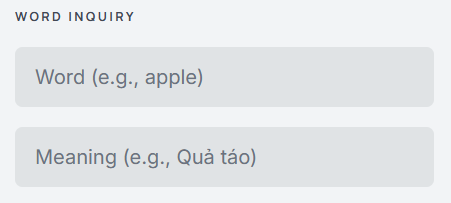
\includegraphics[width=0.8\textwidth]{images/description/word_inquiry.png}
    \caption{Khu vực Word Inquiry}
\end{figure}

\begin{itemize}
    \item \textbf{Bước 1}: Tại vùng Word Inquiry, nhập lần lượt từ vựng và nghĩa của từ.
\end{itemize}

\begin{figure}[H]
    \centering
    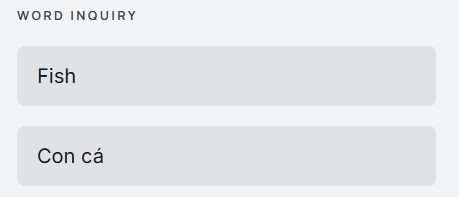
\includegraphics[width=0.8\textwidth]{images/description/enter_word_inquiry.png}
    \caption{Ví dụ nhập thêm mới từ vựng}
\end{figure}

\begin{itemize}
    \item \textbf{Bước 2}: Nhấn nút \textbf{New Entry}.
\end{itemize}

Kết quả: Từ vừa thêm xuất hiện với trạng thái ``THÀNH CÔNG". Quan trọng hơn, biểu đồ Radix Trie sẽ tự động vẽ thêm các nhánh/Node mới đại diện cho từ vừa nhập.

\subsection{Tra cứu từ vựng}
\begin{itemize}
    \item \textbf{Bước 1}: Nhập từ cần tìm vào ô nhập từ.
    \item \textbf{Bước 2}: Nhấn nút Search (biểu tượng kính lúp).
\end{itemize}

\begin{figure}[H]
    \centering
    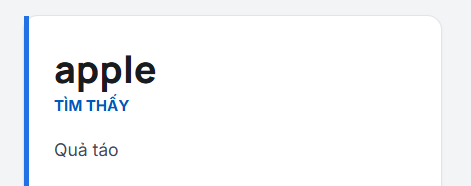
\includegraphics[width=0.8\textwidth]{images/description/find_word.png}
    \caption{Kết quả khi tìm kiếm thành công}
\end{figure}

Kết quả: Hệ thống sẽ truy vấn và lấy nghĩa từ Java Database, hiển thị kết quả và trạng thái ``TÌM THẤY" ngay phía dưới form nhập liệu.

\subsection{Xóa từ vựng}
\begin{itemize}
    \item \textbf{Bước 1}: Nhập từ cần xóa vào ô nhập liệu.
    \item \textbf{Bước 2}: Nhấn nút biểu tượng thùng rác.
\end{itemize}

\begin{figure}[H]
    \centering
    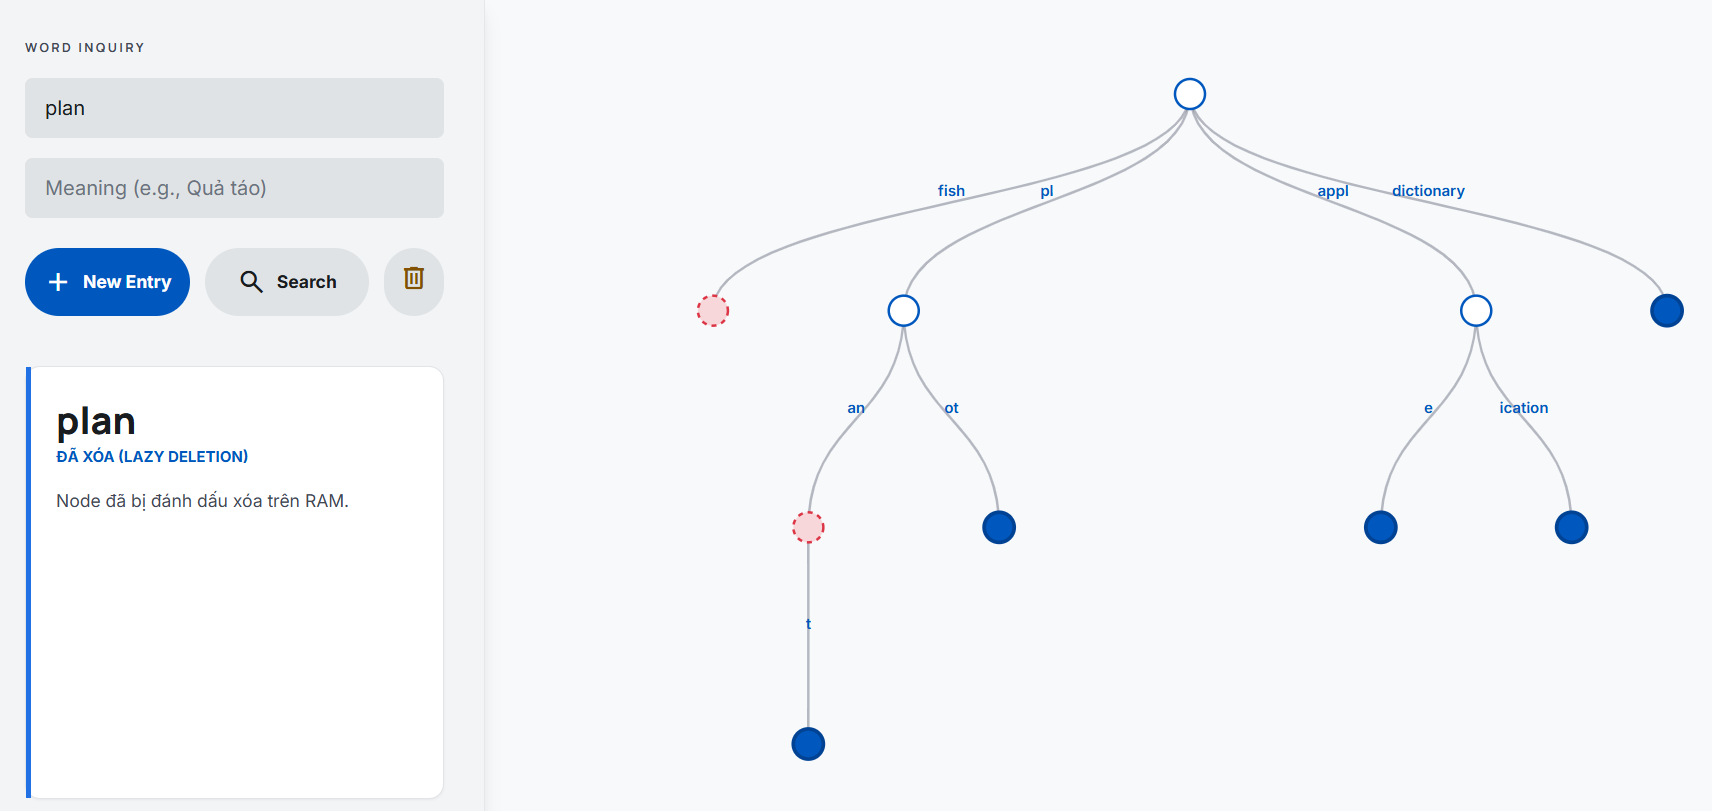
\includegraphics[width=0.8\textwidth]{images/description/delete_a_word.png}
    \caption{Kết quả xóa một từ}
\end{figure}

Kết quả: Hệ thống báo ``ĐÃ XÓA (Lazy Deletion)". Quan sát biểu đồ cây: Node chứa từ vừa xóa không biến mất mà sẽ chuyển sang trạng thái bị vô hiệu hóa.

\end{document}